\documentclass[12pt,fleqn]{article}\usepackage{../../common}
\begin{document}
Ders 7

Vektör uzaylarından, özellikle sıfır uzayından (nullspace), ve kolon
uzayından bahsettik, şimdi bu uzayların içindeki vektörleri nasıl
bulacağımızı, nasıl hesaplayacağımızı göreceğiz. Yani önceki derste
gördüğümüz tanımları bu derste algoritmaya dönüştüreceğiz. $Ax=0$'i çözen
algoritma nedir, mesela. Örnek üzerinde görelim,

$$ 
A = 
\left[\begin{array}{cccc}
1 & 2 & 2 & 2  \\
2 & 4 & 6 & 8 \\
3 & 6 & 8 & 10
\end{array}\right]
 $$

İlk bakışta gözüme çarpan 2. kolon 1. kolonun bir katı. Ya da 2. kolon
1. ile ``aynı yönde'', bu iki kolon ``bağımsız değil''. Tabii bu bilgileri
çözüm sırasında da algoritmanın bir yan etkisi olarak keşfetmeyi
bekleriz. Satırlara bakıyorum, 1. ve 2. toplamı 3. ile aynı, yani 3. satır
bağımsız değil. Tüm bunlar eliminasyonun yan ürünleri olarak bulunmalılar.

Ana algoritmamız eliminasyon olacak, ama onun dikdörtgensel koşula adapte
edilmiş hali, pivotta sıfır var ise durmadan çözüme devam ediyoruz, vs.

Eliminasyon sırasında yapılan işlemler sıfır uzayını değiştirmez. Değil mi?
Bu önemli. Bir denklem sisteminde bir denklemin (satırın) bir katını bir
diğer denklemden çıkartıyorsam bu nihai çözümü değiştirmez, çünkü denklem
sistemi bir bütün olarak değişmemiştir. Satır uzayı değişmez, ama dikkat,
kolon uzayı değişir. Eliminasyonun neyi değiştirdiği neyi değiştirmediğini
bilmek lazım. 

İlk pivot'tan başlayalım (paranteze alınmış olan öğe)

$$ 
\left[\begin{array}{cccc}
(1) & 2 & 2 & 2  \\
2 & 4 & 6 & 8 \\
3 & 6 & 8 & 10
\end{array}\right]
 $$

Pivot satırını 2 ile çarpıp 2. satırdan çıkartıyoruz. Sonra pivot satırını
3 ile çarpıp 3. satırdan çıkartıyoruz. Sonuç

$$ 
\left[\begin{array}{cccc}
1 & 2 & 2 & 2  \\
0 & 0 & 2 & 4 \\
0 & 0 & 2 & 4
\end{array}\right]
 $$

Şimdi sonraki pivot'u arıyoruz, normal durumda bu pivot

$$ 
\left[\begin{array}{cccc}
1 & 2 & 2 & 2  \\
0 & (0) & 2 & 4 \\
0 & 0 & 2 & 4
\end{array}\right]
 $$

olurdu. Ama orada sıfır var, o zaman bir alttaki satıra bakıyoruz, ki
umuyoruz ki satır değiş-tokuşu yaparak o noktaya sıfır olmayan bir değer
gelsin. Ama müstakbel pivot'un altındaki hücre de sıfır değerini taşıyor!
Bu bir şeyin işareti aslında.. Neyin? Bu baktığımız kolonun kendinden önce
gelen kolonların bir kombinasyonu olduğunun işareti. Fakat bunun üzerinde
fazla durmaya gerek yok, algoritmik olarak durup düşünmeye gerek yok, eğer
bir pivot'u kullanamıyorsak hemen yana geçeriz, yani

$$ 
\left[\begin{array}{cccc}
1 & 2 & 2 & 2  \\
0 & 0 & (2) & 4 \\
0 & 0 & 2 & 4
\end{array}\right]
 $$

Şimdi 2. satırı 3. satırdan çıkartmak yeterli. Sonuç altta. Bu matrise $U$
diyebiliriz, gerçi tam üstüçgensel (uppertriangular) sayılmaz, çünkü sıfır
dengesi tam değil, ama basamaklı (echelon) formda, ``hafiften''
üstüçgensel. Tüm pivot'ları gösterirsek,

$$ 
U = 
\left[\begin{array}{cccc}
(1) & 2 & 2 & 2  \\
0 & 0 & (2) & 4 \\
0 & 0 & 0 & 0
\end{array}\right]
 $$

İki tane pivot var; ve bu iki sayısı bu matris hakkında önemli bir bulguya
işaret ediyor, bu matrisin kertesi (rank) 2. Kerte bir matrisin pivot
sayısıdır. 

Bu noktada geriye sokmak (backsubstitution) ile sonucu elde
edebiliriz. Tabii $Ax=0$'in bir sonucu vardır, değil mi? Evet, ki bu
beklenir çünkü elde 3 denklem ve 4 bilinmeyen var, bu sistemden ``bir''
çözüm çıkması normal. Şimdi onları bulmak istiyorum.

Bu çözümleri bulurken kritik adım şu, ki bu adıma ``pivot kolonlarını /
değişkenlerini ayırma'' adı veriyoruz. Pivot kolonları pivot hücrelerinin
olduğu kolonlar ki bunlar 1. ve 3. kolonlar, ve ``serbest kolonlar'' ki
bunlar geri kalanları, yani 2. ve 4. Niye bu isimleri kullandım, özellikle
pivot olmayan kolonlara niye ``serbest'' adını verdim?

Şimdi $Ux=0$'nun çözümünü bulma bağlamında düşünelim. Bu durumda
$x_2,x_4$'a istediğim değeri atayabilirim. Belki cebirsel olarak tüm
denklemleri görmek daha faydalı olur, $Ux=0$'i şöyle yazabiliriz, 

$$ x_1 + 2x_2 + 2x_3 + 2x_4 = 0 $$

$$ 2x_3 + 4x_4 = 0 $$

Ve daha önce dediğimiz gibi bu denklem sistemini geriye sokma yöntemi ile
çözebiliriz, bunlar bildiğimiz şeyler. Yeni olan, elimizde serbest
değişkenler olması, ki bu değişkenlere herhangi bir değer verebiliyorum. Ve
ben şimdi, onlara sistematik olarak ``belli'' değerler atayacağım (herhangi
bir değer olabildiklerine görelim, istediğim değeri atayabilirim), mesela

$$ x = 
\left[\begin{array}{r}
\\
1\\
\\
0
\end{array}\right]
 $$

Yani $x_2=1,x_4=0$ seçtim. Şimdi üstteki 2. formülde $x_4=0$ geriye
koyarsam, $x_3=0$ elde ederim. $x_2=1$ ise, $x_1=-2$. Böylece tamamlanmış $x$,

$$ x = 
\left[\begin{array}{r}
-2\\
1\\
0\\
0
\end{array}\right]
 $$

İşte sıfır uzayında bir vektör bu, çünkü bu $Ax=0$'in çözümlerinden biri. 

Başka hangi çözümler olabilir? Elimizdeki çözümden daha fazla çözüm
üretebilir miyiz? Evet. Üstteki vektörü katlarını alırsak elde edilen
vektörler de sıfır uzayındadır, bir $c$ sabiti kullanalım,

$$ x = 
c \cdot 
\left[\begin{array}{r}
-2\\
1\\
0\\
0
\end{array}\right]
 $$

Bu bize 4 boyutlu uzayda olan bir çizgiyi tarif ediyor. Peki sıfır
uzayının tamamını tarif etmiş olduk mu? Hayır. Çünkü iki tane serbest
değişkenim vardı, onlar için belli bir seçim yaptım. Ama şöyle bir seçim de
yapabilirdim,


$$ x = 
\left[\begin{array}{r}
\\
0\\
\\
1
\end{array}\right]
 $$

Yani $x_2=0,x_4=1$. Bu yeni değerleri geri koyalım; $x_3=-2$, ve 1. denklem
bize $x_1=2$ verir. Hepsi (ve bir $d$ sabiti üzerinden),

$$ x = d \cdot 
\left[\begin{array}{r}
2\\
0\\
-2\\
1
\end{array}\right]
 $$

Terminoloji; üstte belli değerler üzerinden elde ettiğim iki çözüme ``özel
çözümler'' ismi veriyorum, çünkü kendi seçtiğim belli ``özel'' değerler
üzerinden o çözümlere eriştim. 

Nihai çözüm, yani sıfır uzayı üstte hesapladığım iki özel çözümün tüm
lineer kombinasyonları olacaktır. 

Soru: serbest değişken sayısı nereden gelir? Kerte (rank) $r$ ise, kolon boyutu
$n$ olan matris için $n-r = 4-2 = 2$ serbest değişken vardır. Kertenin kolon
boyutundan az olması o matrisin sıfır uzayının büyüklüğü hakkında bir işaret
yani.

Azaltılmış Basamaklı (Reduced Echelon) Matris 

Eliminasyon sonrası elde ettiğimiz matrisi hatırlarsak,

$$ 
\left[\begin{array}{cccc}
1 & 2 & 2 & 2  \\
0 & 0 & 2 & 4 \\
0 & 0 & 0 & 0
\end{array}\right]
 $$

ki bu matris basamaklı, üstüçgensel sayılabilecek bir matristir. 3. satırın
tamamen sıfır olduğuna dikkat edelim, bu oldu çünkü orijinal matriste
3. satır, 1. ve 2. satırların bir kombinasyonu idi ve eliminasyon bu durumu
keşfetti, üstteki 3. satır bu sebeple tamamen sıfır haline geldi. 

Neyse, şimdi bu matrisi biraz daha temizlemek istiyorum. Ne yapabilirim? 

Eliminasyon işlemini yukarı doğru uygulayamaz mıyım? Böylece pivotların
üstünde de, altında olduğu gibi, sıfır değerleri gelebilir - ki bu
azaltılmış basamaklı matrislerin tanımı zaten; bu matrislerde pivotların
hem altında hem üstünde sıfır vardır.

İlerleyelim, 2. satırı 1. satırdan çıkartırsam, 

$$ 
\left[\begin{array}{cccc}
(1) & 2 & 0 & -2  \\
0 & 0 & (2) & 4 \\
0 & 0 & 0 & 0
\end{array}\right]
 $$

Yeni bir sıfır elde etmiş olduk (pivotlar parantezde). Bu arada
pivotlarda hep 1 sayısı görmek istiyorum, 2. satırı 2 ile bölebilirim, bu
denklem sistemini değiştirmez, o zaman

$$ R = 
\left[\begin{array}{cccc}
(1) & 2 & 0 & -2  \\
0 & 0 & (1) & 2 \\
0 & 0 & 0 & 0
\end{array}\right]
 $$

Bu formdaki bir matrise azaltılmış satır basamaklı formu (reduced row
echelon form -rref-) adı veriliyor. Python \verb!sympy! paketindeki
\verb!rref! çağrısı bu çözümü yapar.

\begin{minted}[fontsize=\footnotesize]{python}
import sympy
A = sympy.Matrix([[1., 2., 2., 2. ],
                 [2., 4., 6., 8. ],
                 [3., 6., 8., 10.]] )
print A.rref()[0]
\end{minted}

\begin{verbatim}
[1.0, 2.0,   0, -2.0]
[  0,   0, 1.0,  2.0]
[  0,   0,   0,    0]
\end{verbatim}

$R$ olabilecek en özet bilgiyi içeriyor. Pivot kolonları 1,2 görülüyor,
pivot satırları 1,2 aynı şekilde. Bu arada eğer pivot kolon ve satırları
dışarı çekmiş olsam, bu matris bir birim (identity) matrisi olurdu. 

Eğer $Ux=0$ yerine $Rx=0$'i görmek istersem, 


$$ x_1 + 2x_2 - 2x_4 = 0 $$

$$ x_3 + 2x_4 = 0 $$

Umarım anlaşılıyordur, $Ax=0$ ile başladık, sonra ``orta nokta'' olarak
görebileceğimiz $Ux=0$'i elde ettik, ve şimdi üstte $Rx=0$'i
görüyoruz... Bu sistemlerin hepsi birbiri ile eşdeğerdir, çünkü birinden
diğerine giderken sistemi bozmadık. Bir satırı bir şey ile çarpıp bir
diğerinden çıkartmak gibi işlemler uyguladık ki bu tür işlemler denklem
sistemini bozmuyor.

Tüm çözümler, 

$$ 
x = 
c \cdot 
\left[\begin{array}{r}
-2\\ 1\\ 0\\ 0
\end{array}\right]
+
d \cdot 
\left[\begin{array}{r}
2\\ 0\\ -2\\ 1
\end{array}\right]
 $$

Önemli nokta: üstteki serbest değişkenlerin değerleri $R$'içindeki
değerlerin negatifi alınmış hali. Niye?

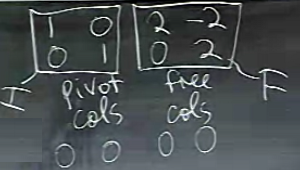
\includegraphics[height=4cm]{7_01.png}

Eğer pivot kolonlarını bir araya, serbest (free) kolonlarını biraraya
koyarsam üstteki şekil ortaya çıkar. 

$$ R = 
\left[\begin{array}{cccc}
I & F   \\
0 & 0
\end{array}\right]
 $$

Üstte görülen oldukça tipik bir rref matrisidir. $I$'nin boyutları $r
\times r$, çünkü $r$ tane pivot kolonu var, $F$'nin kolon sayısı $n-r$,
çünkü o kadar serbest değişken var. Peki özel çözümler nedir? Madem matris
bir blok matris halinde (yani $I,F$ bloklar olarak bir diğerinin içinde),
eh o zaman $Rx = 0$'in çözümlerini direk bu matris üzerinden elde
edebilirim. Bir sıfır uzayı matrisi oluşturacağım ki bu matrisin kolonları
özel çözümüm olacak. Bu matrise $N$ diyeyim, öyle ki $RN = 0$ olsun,

$$ 
N = 
\left[\begin{array}{rr}
-F & I
\end{array}\right]
$$

Eksi işaret nereden geldi? $Rx=0$'i şöyle gösterirsek,

$$ 
\left[\begin{array}{rr}
I & F
\end{array}\right]
\left[\begin{array}{l}
x_{pivot} \\ x_{serbest} 
\end{array}\right] = 0
 $$

Açarsak, 

$x_{pivot} = -F x_{serbest}$

Yeni bir örnek çözelim. 

$$ 
A = \left[\begin{array}{rrr}
1 & 2 & 3 \\
2 & 4 & 6 \\
2 & 6 & 8 \\
2 & 8 & 10 \\
\end{array}\right]
 $$

Çözmeye başlamadan önce hemen ilk bakışla ne gördüğümüzü söyleyelim; Kaç
tane pivot olmasını, yani kaç tane kolonun pivot'unun olmasını
beklemeliyiz? Bu matriste üç tane kolon var, peki üç tane pivot elde edecek
miyiz? Hayır, çünkü 3. kolon 1. ve 2. kolonların bir toplamı. Bu kolon yeni
bir enformasyon sağlamıyor, yani ``bağımsız değil''. Çözüm sırasında benim
beklentim şöyle, 1. ve 2. kolon pivot olacak, ama 3. bağımlı olduğu için
serbest kolon olacak. Eliminasyon bunu bulmalı. 

2 tane 1. satırı 2., 3. ve 4. satırdan çıkartırsam, 

$$ 
\left[\begin{array}{rrr}
1 & 2 & 3 \\
0 & 0 & 0 \\
0 & 2 & 2 \\
0 & 4 & 4 \\
\end{array}\right]
 $$

Şimdi sonraki pivot'a gidiyorum, yani (2,2) kordinatına, orada sıfır
var. Altına gidiyorum, orada 2 var. Demek ki satır değiş-tokuşu lazım, bunu
yaptıktan sonra istediğim noktada pivot var,

$$ 
\left[\begin{array}{ccc}
(1) & 2 & 3 \\
0 & (2) & 2 \\
0 & 0 & 0 \\
0 & 4 & 4 \\
\end{array}\right]
 $$

2. tane 2. satırı 4.'den çıkartıyorum, nihayet $U$'yu elde ediyorum,

$$ 
U = \left[\begin{array}{rrr}
1 & 2 & 3 \\
0 & 2 & 2 \\
0 & 0 & 0 \\
0 & 0 & 0 \\
\end{array}\right]
 $$

Kerte yine $r=2$. Kaç tane özel çözüm var? $3-2=1$, demek ki 1 tane serbest
kolon var. Özel çözümü bulmak için serbest değişkene 1 değeri veririm, 

Denklem halinde

$$ x_1 + 2x_2 + 3x_3 = 0 $$

$$ 2x_2 + 2x_3 = 0 $$

$x_3=1$ ile başlarsak geriye koyma ile,

$$ x = 
\left[\begin{array}{r}
-1\\
-1\\
1
\end{array}\right]
 $$

Hızlı bir doğrulama yapmak gerekirse, üstteki çözüm ne diyor? $A$'nin
1. ve 2. kolonundan -1 tane ve 3. kolonundan 1 tane alıp toplarsam sonuç
sıfır olacaktır. Ve hakikaten de bu doğru, zaten problemin başında 1. ve
2. kolonun toplamının 3.'ye eşit olduğunu söylemememiş miydik? Evet.

Tüm çözümler, 

$$ x = 
c \cdot \left[\begin{array}{r}
-1\\
-1\\
1
\end{array}\right]
 $$

Sınavda üstteki çözümü göstermenizi beklerim. Daha ilerideki sınavlarda
sıfır uzayın ``bazını'' soracağım, o zaman $c$ olmadan tek vektörü
verebilirsiniz, ama sıfır uzayını istiyorsam üstteki problem için tüm bir
çizgiyi vermeniz lazım. 

Bu örnekte gidilecek sonraki doğal adım, rref formuna gitmek. 2. satırı
alıp 1. den çıkartabilirim, ve 2. satırı 2'ye bölebilirim, 

$$ 
R = \left[\begin{array}{rrr}
1 & 0 & 1 \\
0 & 1 & 1 \\
0 & 0 & 0 \\
0 & 0 & 0 \\
\end{array}\right]
 $$

$I$ kısmı görülüyor, sol üst köşedeki $2 \times 2$ boyutlu blok
matris. Onun hemen yanındaki $2 \times 1$ boyutlu içinde sadece 1 olan
kısım $F$. Üstte $x$ için gösterdiğimiz bölümde $F$'in negatifi olduğunu
dikkat, yani 

$$ x = 
c \cdot \left[\begin{array}{r}
-F \\
I
\end{array}\right]
 $$

ki $c$'nin çarptığı matris $N$ matrisi, yani sıfır uzayı matrisidir, ki bu
matrisin kolonları bizim özel çözümlerimiz. 

$Ax=0$ hakkında söyleyecek daha fazla bir şey kalmadı sanıyorum. $Ax=b$
konusunda söyleyeceklerimiz daha var, ama bu bir sonraki derste. 


\end{document}




